


\begin{figure}[ht]
\centering
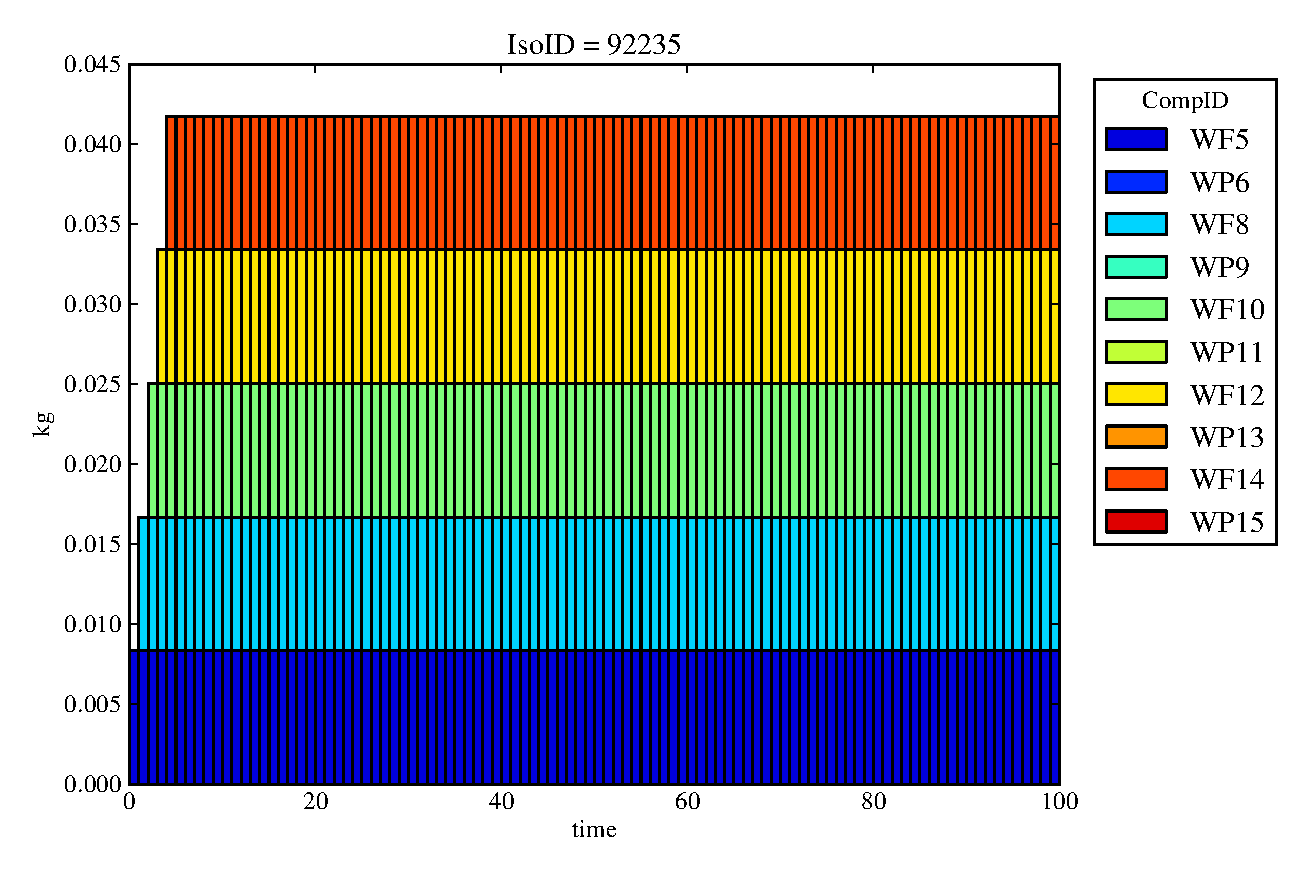
\includegraphics[width=0.8\textwidth]{./chapters/demonstration/base/lpEMII.eps}
\caption[$^{235}U$ residence. Lumped Parameter  Waste Package No Release.]{
For case LPEMII in which total containment in the waste package is assumed 
($F_{d,wp}=0$), $^{235}U$ travels through the waste form component ($F_d = 0.1$) before 
permanent residence in the waste package component.
}
\label{fig:lpEMIIall}
\begin{minipage}[b]{0.45\linewidth}

  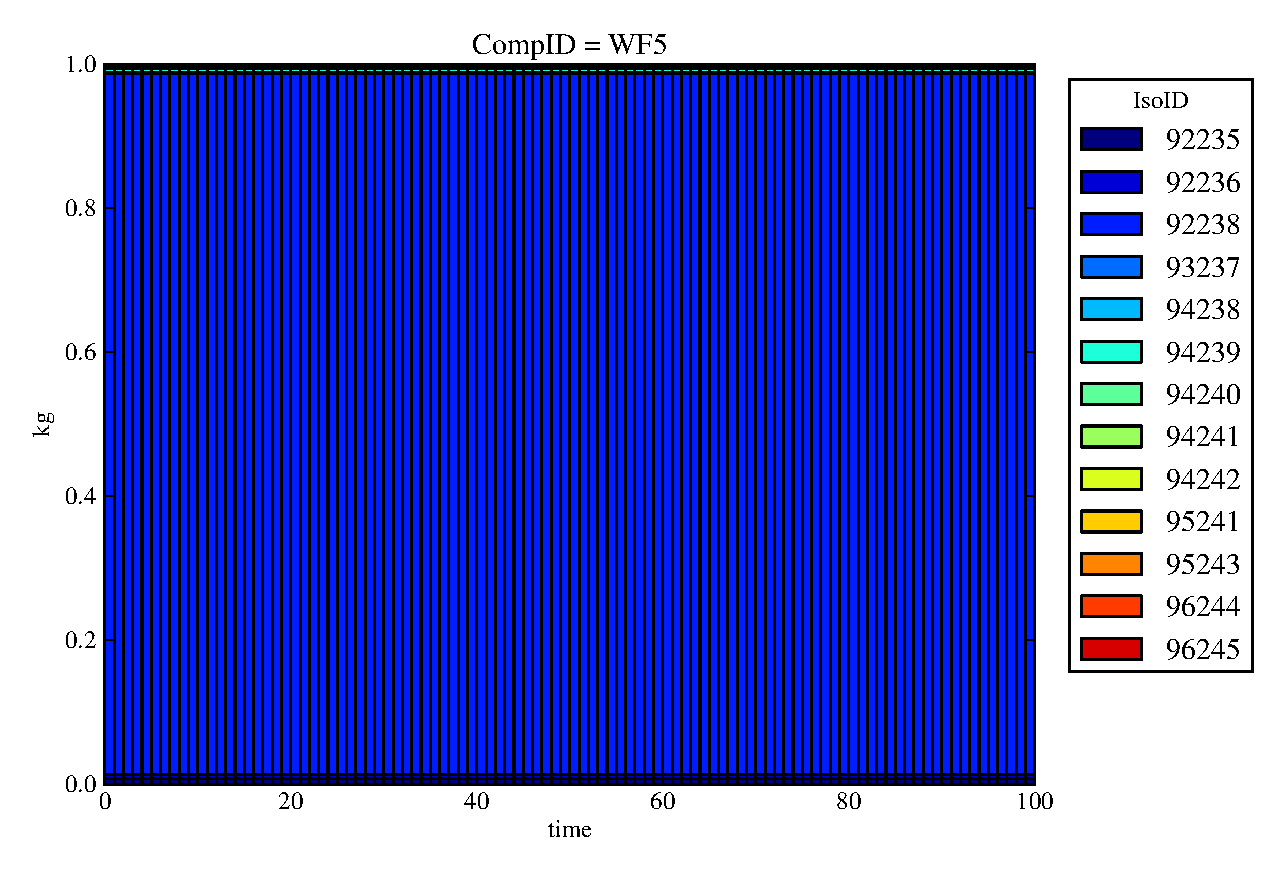
\includegraphics[width=\textwidth]{./chapters/demonstration/base/lpEMII1.eps}
  \caption[LPEMII Waste Form Contaminants.]{
    Waste Form 5 ($F_d = 0.1$) releases material with degradation. 
    }
  \label{fig:lpEMIIwf5}
  
  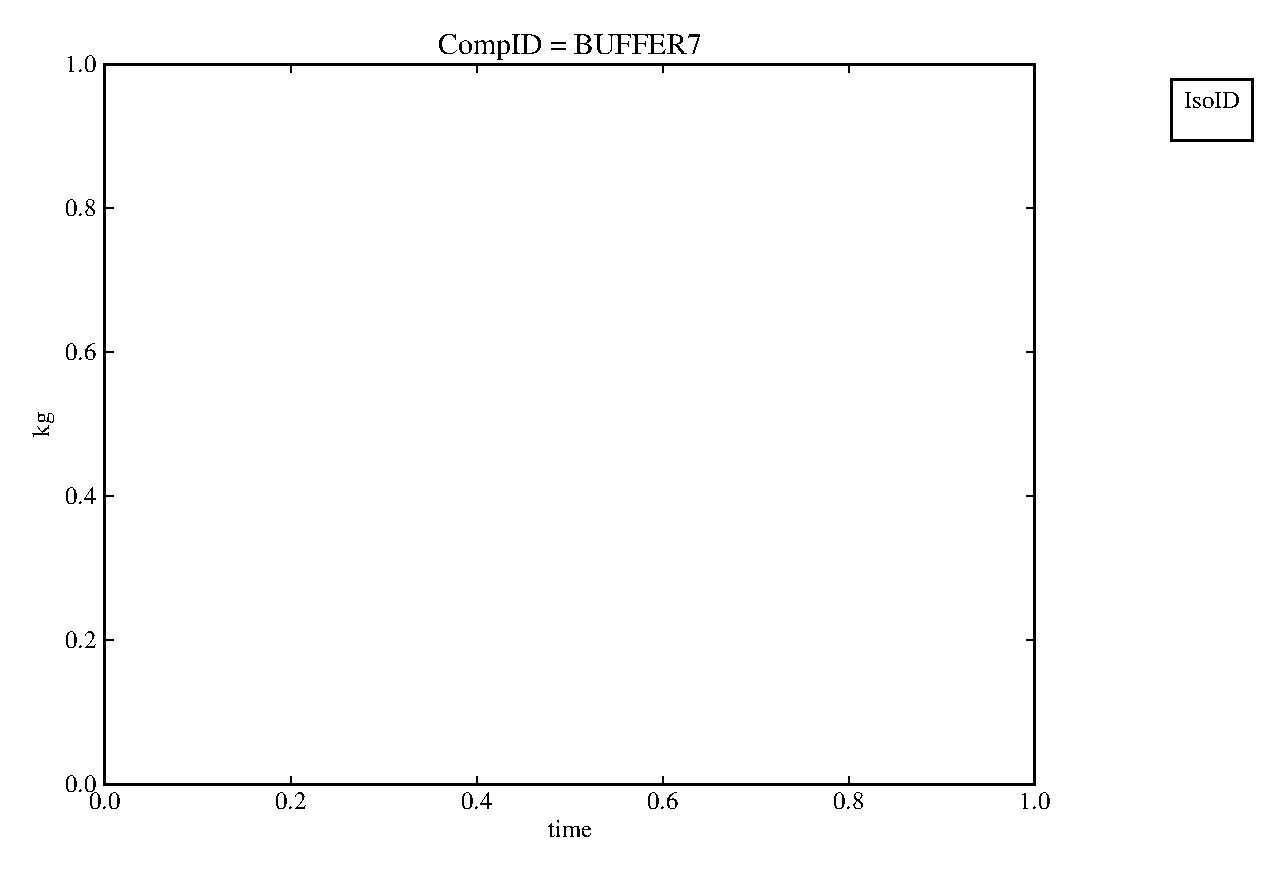
\includegraphics[width=\textwidth]{./chapters/demonstration/base/lpEMII3.eps}
  \caption[Case LPEMII Buffer Contaminants]{
    The Buffer, component 7 ($F_d=0$), acheives total containment.
    }
  \label{fig:lpEMIIbuff}

\end{minipage}
\hspace{0.05\linewidth}
\begin{minipage}[b]{0.45\linewidth}
  \includegraphics[width=\textwidth]{./chapters/demonstration/base/lpEMII2.eps}
  \caption[Case LPEMII Waste Package Contaminants.]{ 
    Waste Package 6 ($F_d = 0.1$) recieves then releases material. 
    }
  \label{fig:lpEMIIwp6}

  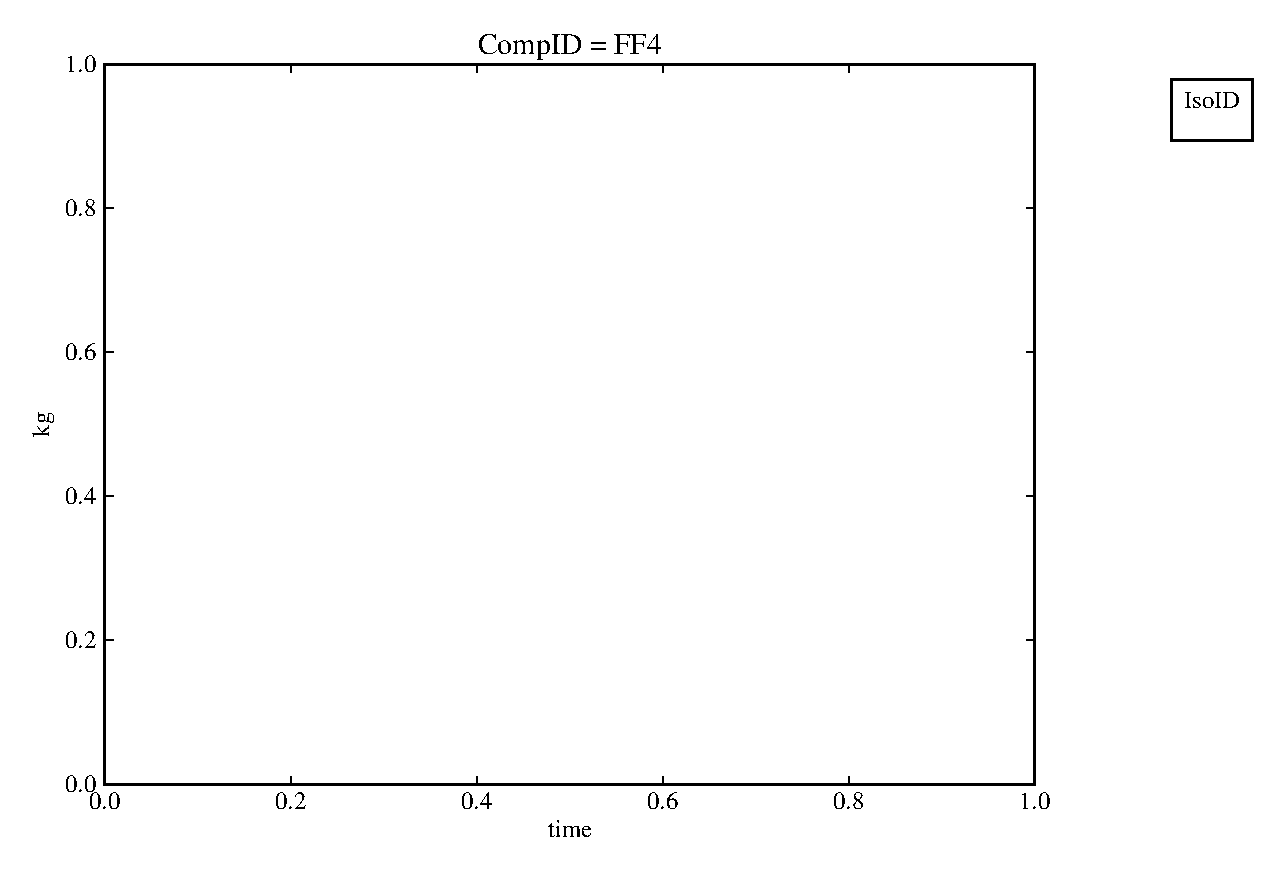
\includegraphics[width=\textwidth]{./chapters/demonstration/base/lpEMII0.eps}
  \caption[Case LPEMII Waste Package Contaminants.]{ 
    The Far Field, component 0 ($F_d = 0.1$), never recieves material.
    }
  \label{fig:lpEMIIff0}


  \end{minipage}
\end{figure}
%\begin{figure}[ht]
%\centering
%\includegraphics[width=0.8\textwidth]{./chapters/demonstration/base/lpEMIII.eps}
%\caption[$^{235}U$ residence. Lumped Parameter  <+Component+> No Release.]{
%For <+CASE+> case in which total containment in the <+component+> is assumed 
%($F_{d,<+comp+>}=0$), $^{235}U$ travels through  components ($F_d = 0.1$) before 
%permanent residence in the <+component+> component.
%}
%\label{fig:lpEMIIIall}
%\begin{minipage}[b]{0.45\linewidth}
%
%  \includegraphics[width=\textwidth]{./chapters/demonstration/base/lpEMIII1.eps}
%  \caption[LPEMIII Waste Form Contaminants.]{
%    Waste Form 5 ($F_d = 0.1$) releases material with degradation. 
%    }
%  \label{fig:lpEMIIIwf5}
%  
%  \includegraphics[width=\textwidth]{./chapters/demonstration/base/lpEMIII3.eps}
%  \caption[Case LPEMIII Buffer Contaminants]{
%    The Buffer, component 7 ($F_d=0$), acheives total containment.
%    }
%  \label{fig:lpEMIIIbuff}
%
%\end{minipage}
%\hspace{0.05\linewidth}
%\begin{minipage}[b]{0.45\linewidth}
%  \includegraphics[width=\textwidth]{./chapters/demonstration/base/lpEMIII2.eps}
%  \caption[Case LPEMIII Waste Package Contaminants.]{ 
%    Waste Package 6 ($F_d = 0.1$) recieves then releases material. 
%    }
%  \label{fig:lpEMIIIwp6}
%
%  \includegraphics[width=\textwidth]{./chapters/demonstration/base/lpEMIII0.eps}
%  \caption[Case LPEMIII Waste Package Contaminants.]{ 
%    The Far Field, component 0 ($F_d = 0.1$), never recieves material.
%    }
%  \label{fig:lpEMIIIff0}
%
%
%  \end{minipage}
%\end{figure}
%\begin{figure}[ht]
%\centering
%\includegraphics[width=0.8\textwidth]{./chapters/demonstration/base/lpEMIV.eps}
%\caption[$^{235}U$ residence. Lumped Parameter  <+Component+> No Release.]{
%For <+CASE+> case in which total containment in the <+component+> is assumed 
%($F_{d,<+comp+>}=0$), $^{235}U$ travels through  components ($F_d = 0.1$) before 
%permanent residence in the <+component+> component.
%}
%\label{fig:lpEMIVall}
%\begin{minipage}[b]{0.45\linewidth}
%
%  \includegraphics[width=\textwidth]{./chapters/demonstration/base/lpEMIV1.eps}
%  \caption[LPEMIV Waste Form Contaminants.]{
%    Waste Form 5 ($F_d = 0.1$) releases material with degradation. 
%    }
%  \label{fig:lpEMIVwf5}
%  
%  \includegraphics[width=\textwidth]{./chapters/demonstration/base/lpEMIV3.eps}
%  \caption[Case LPEMIV Buffer Contaminants]{
%    The Buffer, component 7 ($F_d=0$), acheives total containment.
%    }
%  \label{fig:lpEMIVbuff}
%
%\end{minipage}
%\hspace{0.05\linewidth}
%\begin{minipage}[b]{0.45\linewidth}
%  \includegraphics[width=\textwidth]{./chapters/demonstration/base/lpEMIV2.eps}
%  \caption[Case LPEMIV Waste Package Contaminants.]{ 
%    Waste Package 6 ($F_d = 0.1$) recieves then releases material. 
%    }
%  \label{fig:lpEMIVwp6}
%
%  \includegraphics[width=\textwidth]{./chapters/demonstration/base/lpEMIV0.eps}
%  caption[Case LPEMIV Waste Package Contaminants.]{ 
%    The Far Field, component 0 ($F_d = 0.1$), never recieves material.
%    }
%  \label{fig:lpEMIVff0}
%
%
%  \end{minipage}
%\end{figure}

%%%%%%%%%%%%%%%%%%%%%%%%%%%%%%
% DM
%%%%%%%%%%%%%%%%%%%%%%%%%%%%%%

\begin{figure}[ht]
\centering
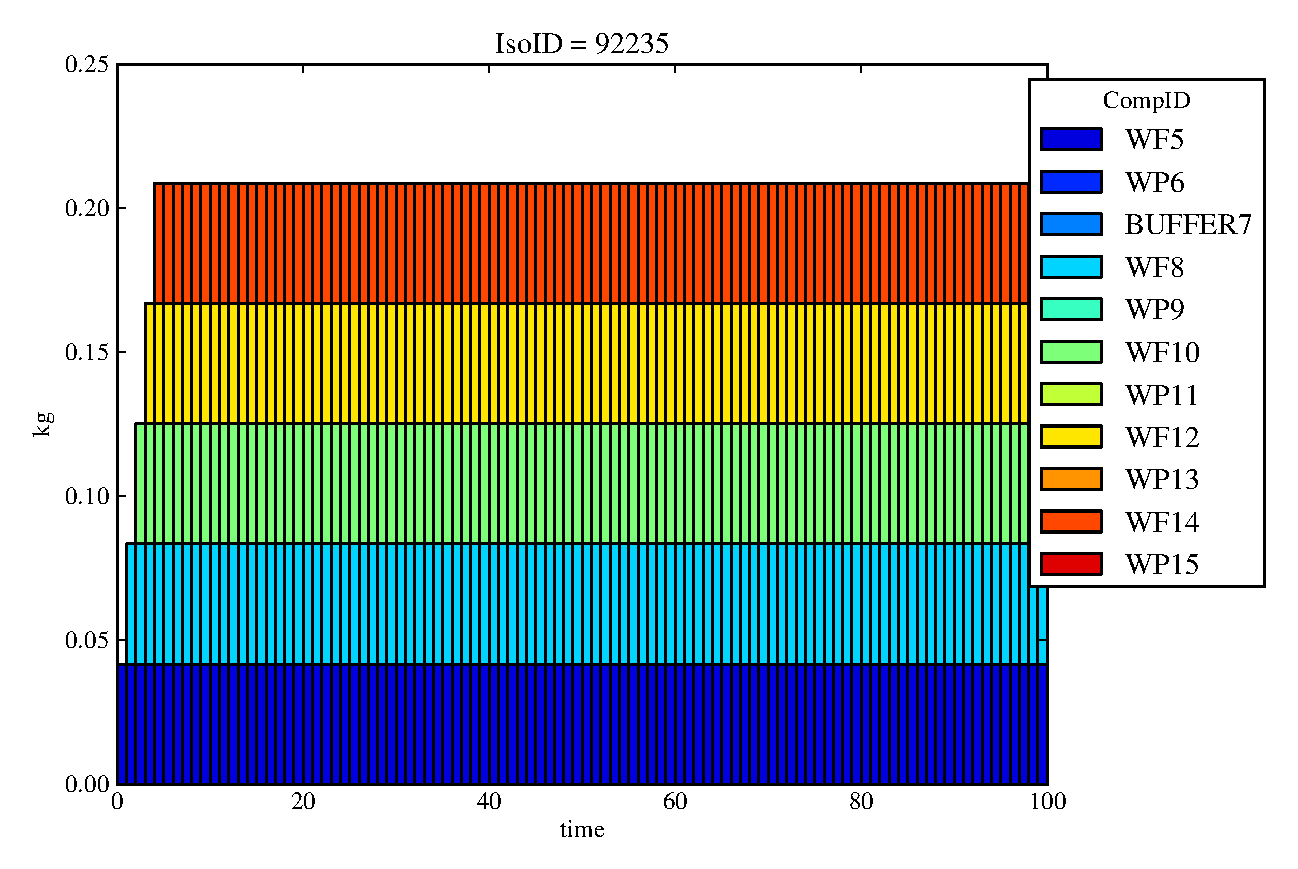
\includegraphics[width=0.8\textwidth]{./chapters/demonstration/base/lpDMII.eps}
\caption[$^{235}U$ residence. Lumped Parameter  DM Waste Package No Release.]{
For LPDMII case in which total containment in the waste package is assumed 
($F_{d,wp}=0$), $^{235}U$ travels through the waste form component ($F_d = 0.1$) before 
permanent residence in the waste package component.
}
\label{fig:lpDMIIall}
\begin{minipage}[b]{0.45\linewidth}

  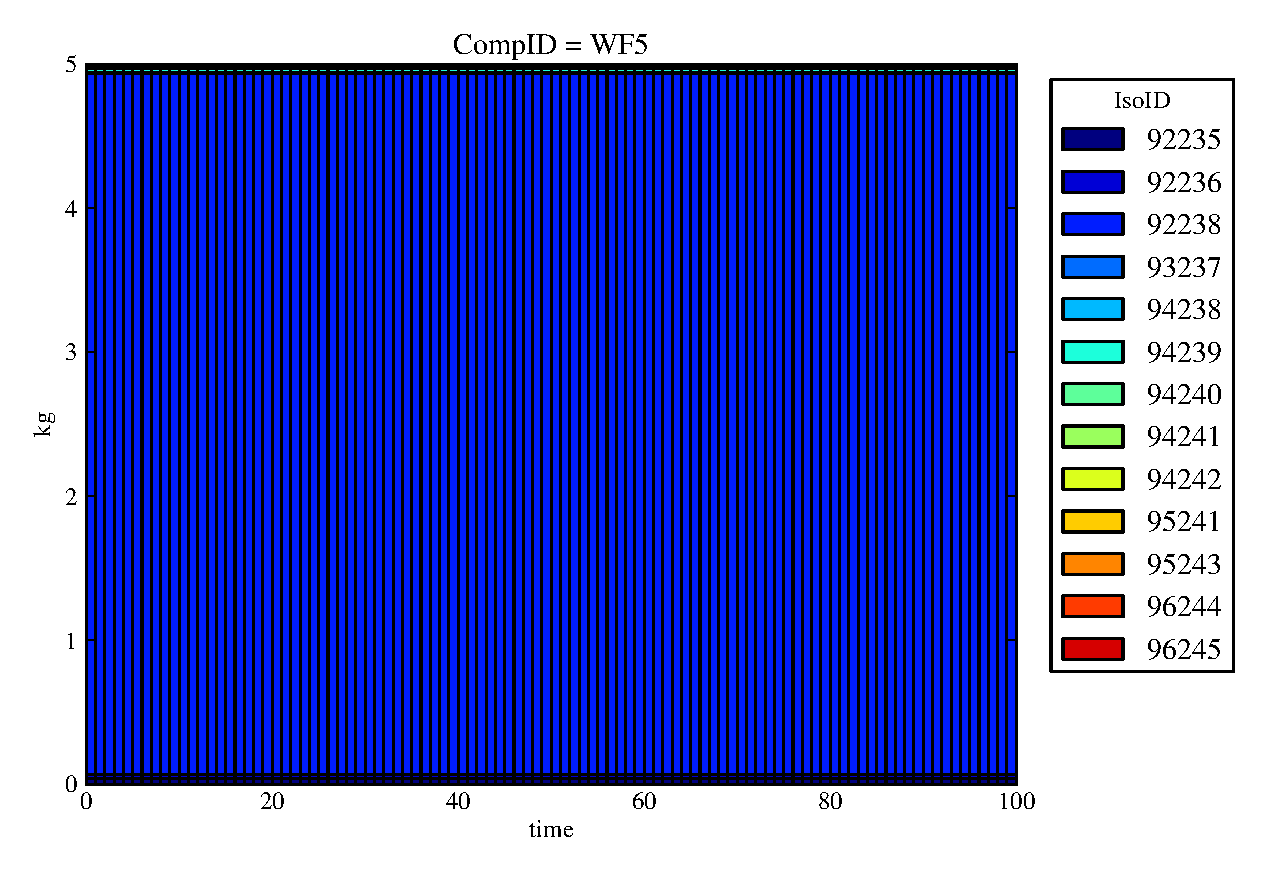
\includegraphics[width=\textwidth]{./chapters/demonstration/base/lpDMII1.eps}
  \caption[LPDMII Waste Form Contaminants.]{
    Waste Form 5 ($F_d = 0.1$) releases material with degradation. 
    }
  \label{fig:lpDMIIwf5}
  
  \includegraphics[width=\textwidth]{./chapters/demonstration/base/lpDMII3.eps}
  \caption[Case LPDMII Buffer Contaminants]{
    The Buffer, component 7 ($F_d=0$), acheives total containment.
    }
  \label{fig:lpDMIIbuff}

\end{minipage}
\hspace{0.05\linewidth}
\begin{minipage}[b]{0.45\linewidth}
  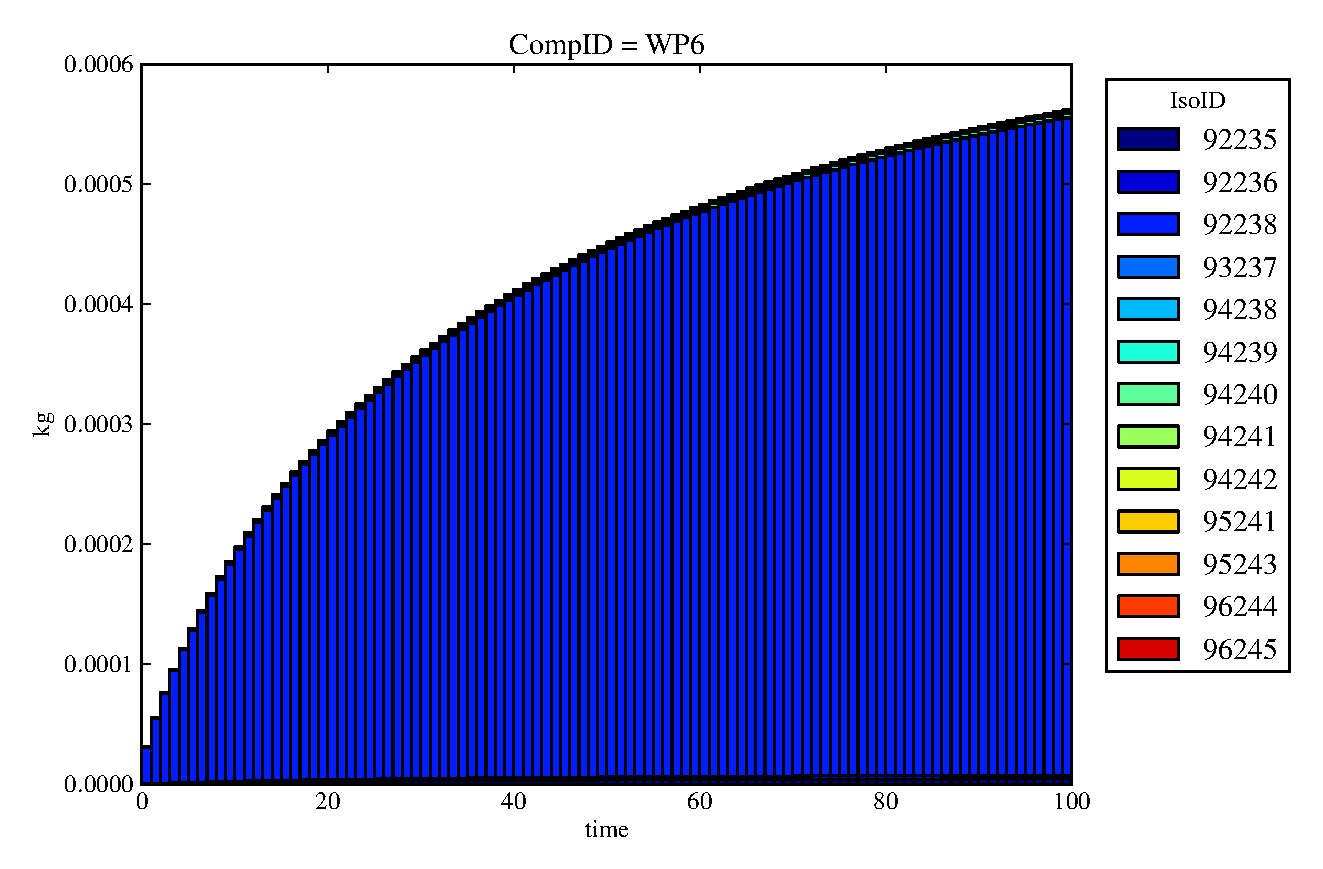
\includegraphics[width=\textwidth]{./chapters/demonstration/base/lpDMII2.eps}
  \caption[Case LPDMII Waste Package Contaminants.]{ 
    Waste Package 6 ($F_d = 0.1$) recieves then releases material. 
    }
  \label{fig:lpDMIIwp6}

  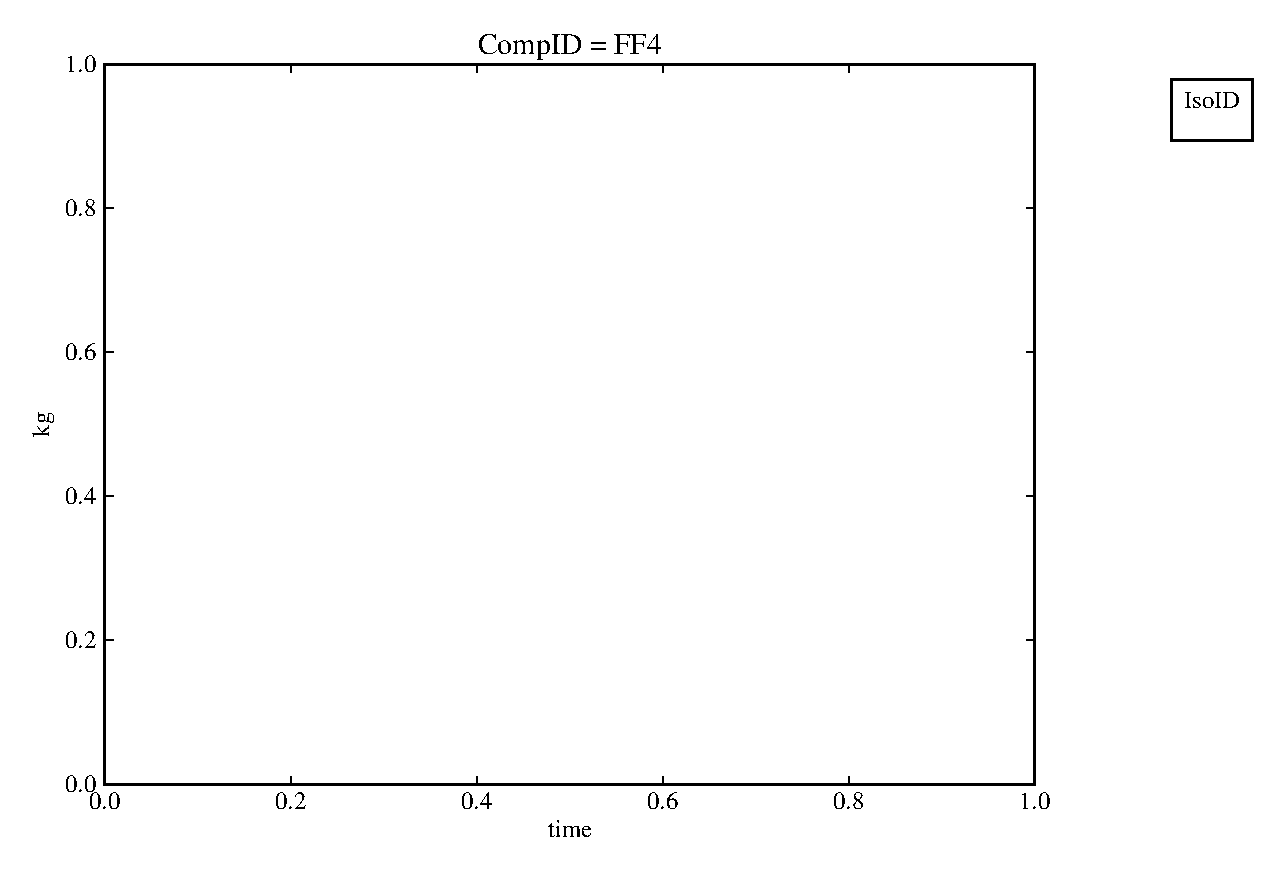
\includegraphics[width=\textwidth]{./chapters/demonstration/base/lpDMII0.eps}
  \caption[Case LPDMII Waste Package Contaminants.]{ 
    The Far Field, component 0 ($F_d = 0.1$), never recieves material.
    }
  \label{fig:lpDMIIff0}


  \end{minipage}
\end{figure}
%\begin{figure}[ht]
%\centering
%\includegraphics[width=0.8\textwidth]{./chapters/demonstration/base/lpDMIII.eps}
%\caption[$^{235}U$ residence. Lumped Parameter  <+Component+> No Release.]{
%For <+CASE+> case in which total containment in the <+component+> is assumed 
%($F_{d,<+comp+>}=0$), $^{235}U$ travels through  components ($F_d = 0.1$) before 
%permanent residence in the <+component+> component.
%}
%\label{fig:lpDMIIIall}
%\begin{minipage}[b]{0.45\linewidth}
%
%  \includegraphics[width=\textwidth]{./chapters/demonstration/base/lpDMIII1.eps}
%  \caption[LPDMIII Waste Form Contaminants.]{
%    Waste Form 5 ($F_d = 0.1$) releases material with degradation. 
%    }
%  \label{fig:lpDMIIIwf5}
%  
%  \includegraphics[width=\textwidth]{./chapters/demonstration/base/lpDMIII3.eps}
%  \caption[Case LPDMIII Buffer Contaminants]{
%    The Buffer, component 7 ($F_d=0$), acheives total containment.
%    }
%  \label{fig:lpDMIIIbuff}
%
%\end{minipage}
%\hspace{0.05\linewidth}
%\begin{minipage}[b]{0.45\linewidth}
%  \includegraphics[width=\textwidth]{./chapters/demonstration/base/lpDMIII2.eps}
%  \caption[Case LPDMIII Waste Package Contaminants.]{ 
%    Waste Package 6 ($F_d = 0.1$) recieves then releases material. 
%    }
%  \label{fig:lpDMIIIwp6}
%
%  \includegraphics[width=\textwidth]{./chapters/demonstration/base/lpDMIII0.eps}
%  \caption[Case LPDMIII Waste Package Contaminants.]{ 
%    The Far Field, component 0 ($F_d = 0.1$), never recieves material.
%    }
%  \label{fig:lpDMIIIff0}
%
%
%  \end{minipage}
%\end{figure}
%\begin{figure}[ht]
%\centering
%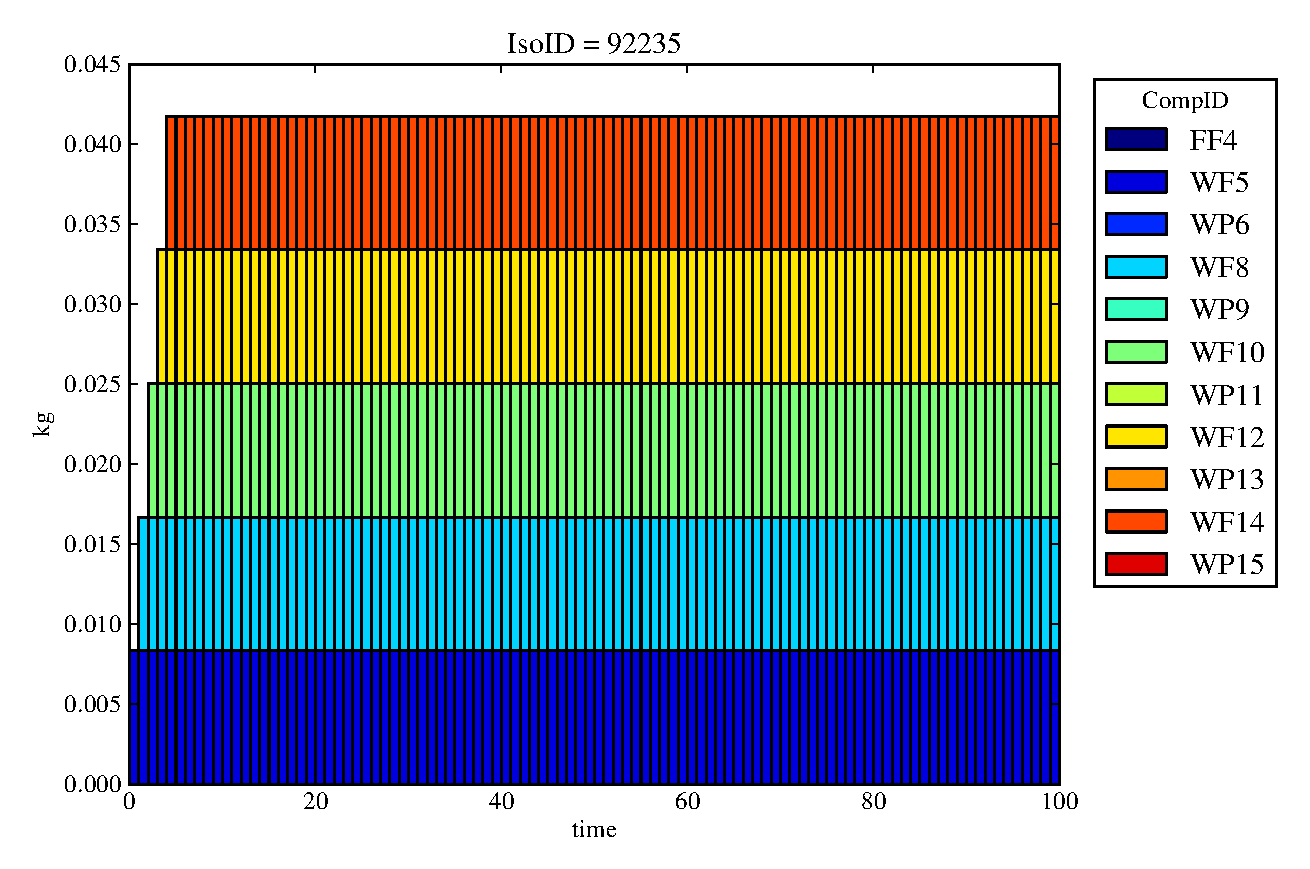
\includegraphics[width=0.8\textwidth]{./chapters/demonstration/base/lpDMIV.eps}
%\caption[$^{235}U$ residence. Lumped Parameter  <+Component+> No Release.]{
%For <+CASE+> case in which total containment in the <+component+> is assumed 
%($F_{d,<+comp+>}=0$), $^{235}U$ travels through  components ($F_d = 0.1$) before 
%permanent residence in the <+component+> component.
%}
%\label{fig:lpDMIVall}
%\begin{minipage}[b]{0.45\linewidth}
%
%  \includegraphics[width=\textwidth]{./chapters/demonstration/base/lpDMIV1.eps}
%  \caption[LPDMIV Waste Form Contaminants.]{
%    Waste Form 5 ($F_d = 0.1$) releases material with degradation. 
%    }
%  \label{fig:lpDMIVwf5}
%  
%  \includegraphics[width=\textwidth]{./chapters/demonstration/base/lpDMIV3.eps}
%  \caption[Case LPDMIV Buffer Contaminants]{
%    The Buffer, component 7 ($F_d=0$), acheives total containment.
%    }
%  \label{fig:lpDMIVbuff}
%
%\end{minipage}
%\hspace{0.05\linewidth}
%\begin{minipage}[b]{0.45\linewidth}
%  \includegraphics[width=\textwidth]{./chapters/demonstration/base/lpDMIV2.eps}
%  \caption[Case LPDMIV Waste Package Contaminants.]{ 
%    Waste Package 6 ($F_d = 0.1$) recieves then releases material. 
%    }
%  \label{fig:lpDMIVwp6}
%
%  \includegraphics[width=\textwidth]{./chapters/demonstration/base/lpDMIV0.eps}
%  caption[Case LPDMIV Waste Package Contaminants.]{ 
%    The Far Field, component 0 ($F_d = 0.1$), never recieves material.
%    }
%  \label{fig:lpDMIVff0}
%
%
%  \end{minipage}
%\end{figure}
%%%%%%%%%%%%%%%%%%%%%%%%%%%%%%%
% PFM
%%%%%%%%%%%%%%%%%%%%%%%%%%%%%%%

\begin{figure}[ht!]
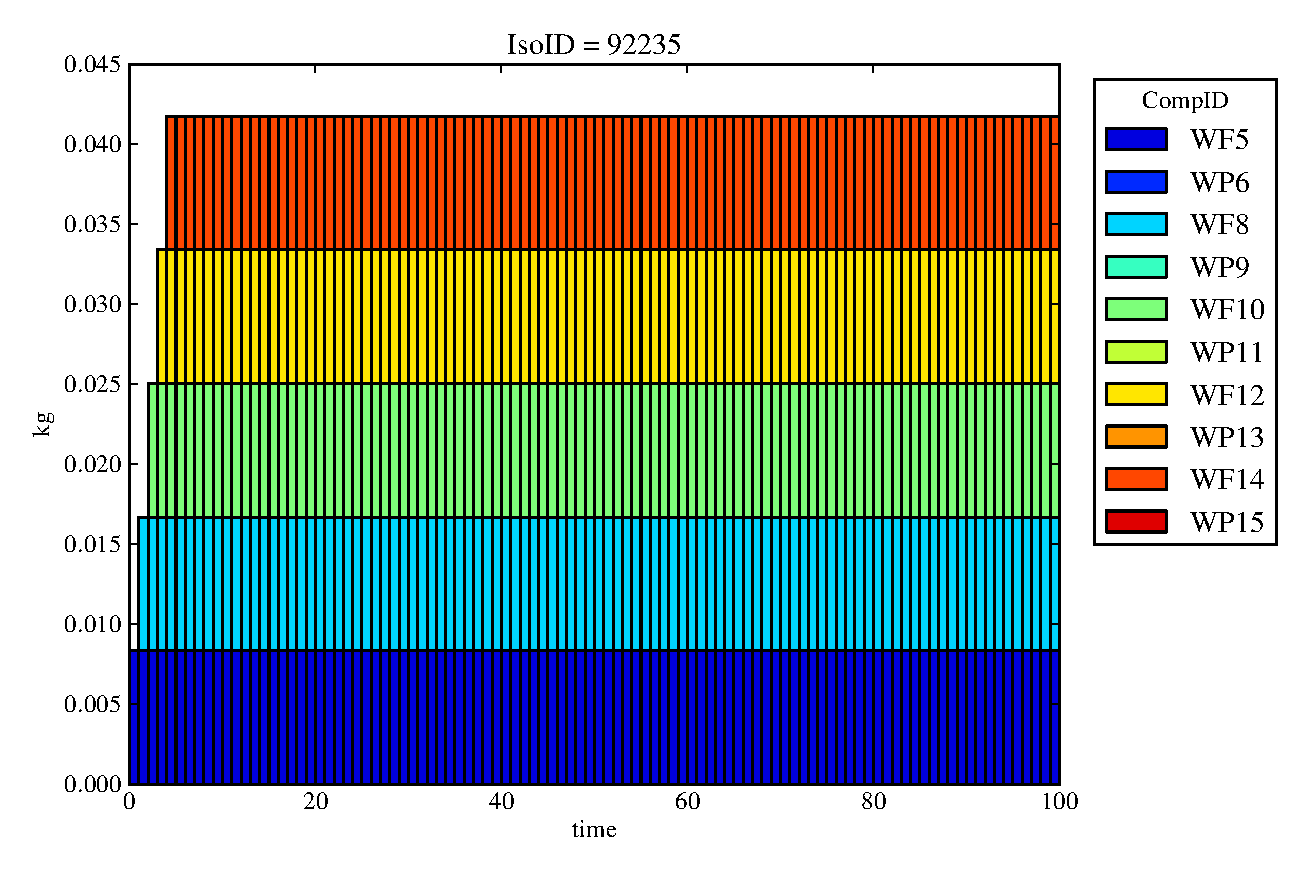
\includegraphics[width=0.8\textwidth]{./chapters/demonstration/base/lpPFMII.eps}
\caption[$^{235}U$ residence. Lumped Parameter PFM Waste Package No Release.]{
For case LPPFMII in which total containment in the waste package is assumed 
($F_{d,wp}=0$), $^{235}U$ travels through the waste form component ($F_d = 0.1$) before 
permanent residence in the waste package component.
}
\label{fig:lpPFMIIall}
\begin{minipage}[b]{0.45\linewidth}
  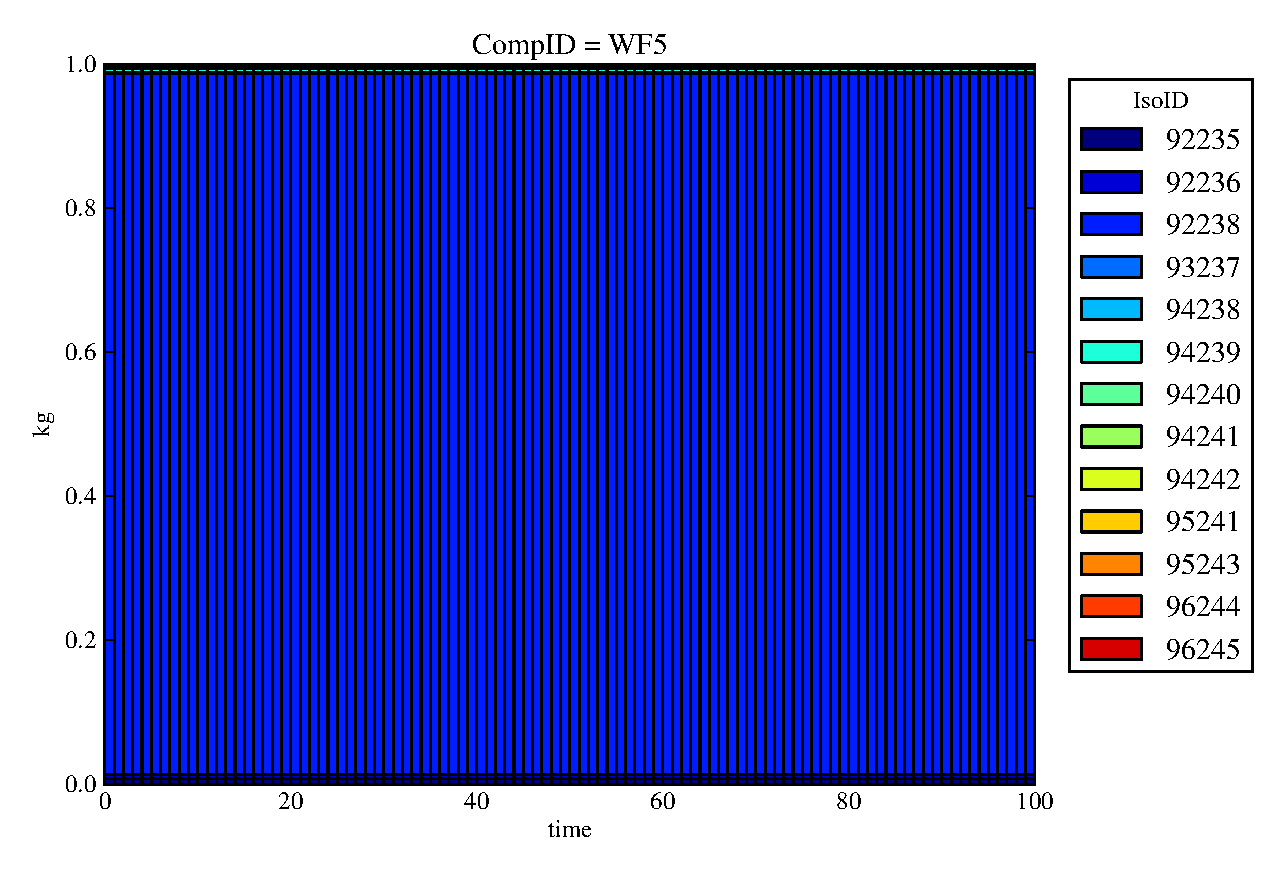
\includegraphics[width=\textwidth]{./chapters/demonstration/base/lpPFMII1.eps}
  \caption[LPPFMII Waste Form Contaminants.]{
    Waste Form 5 ($F_d = 0.1$) releases material with degradation. 
    }
  \label{fig:lpPFMIIwf5}
  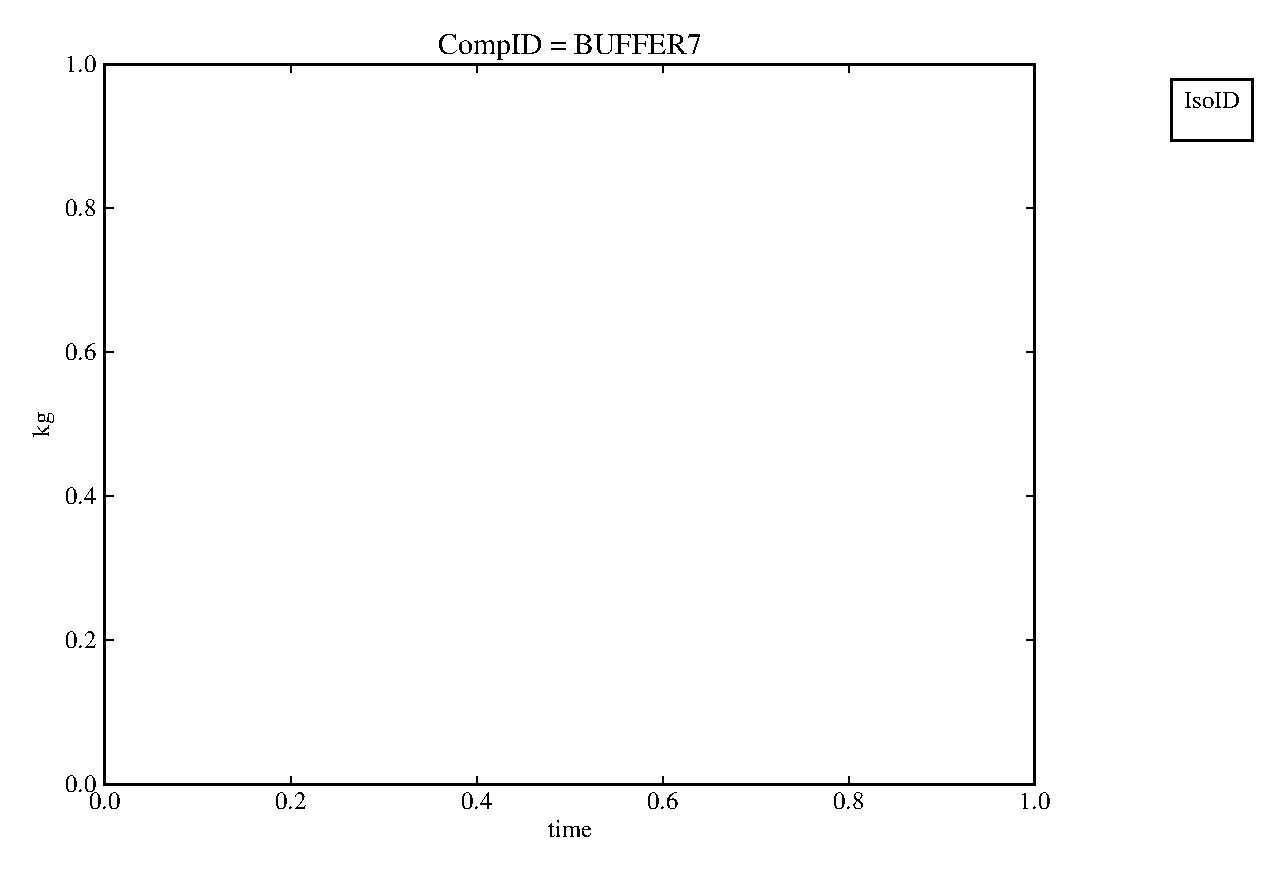
\includegraphics[width=\textwidth]{./chapters/demonstration/base/lpPFMII3.eps}
  \caption[Case LPPFMII Buffer Contaminants]{
    The Buffer, component 7 ($F_d=0$), acheives total containment.
    }
  \label{fig:lpPFMIIbuff}

\end{minipage}
\hspace{0.05\linewidth}
\begin{minipage}[b]{0.45\linewidth}
  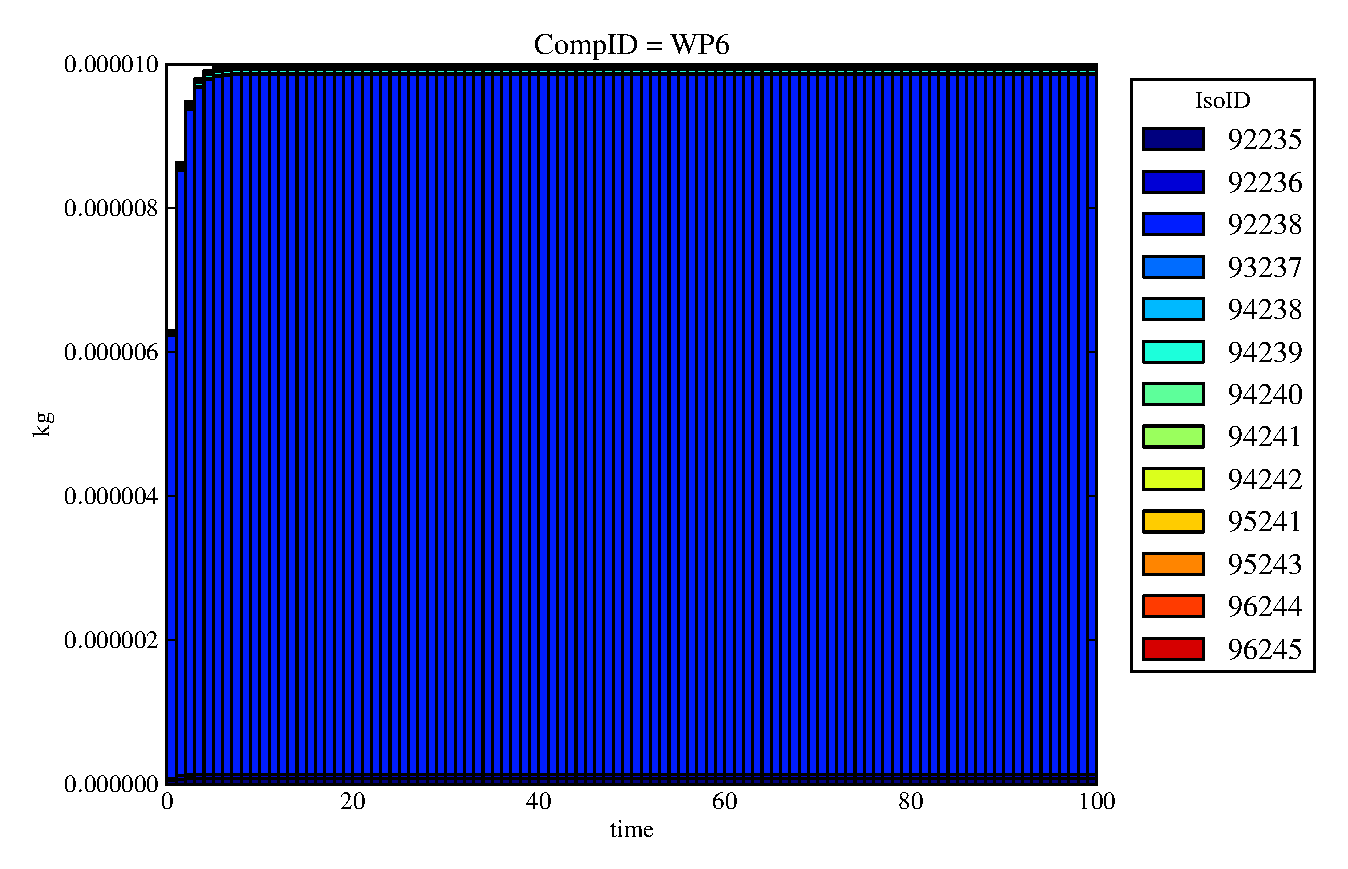
\includegraphics[width=\textwidth]{./chapters/demonstration/base/lpPFMII2.eps}
  \caption[Case LPPFMII Waste Package Contaminants.]{ 
    Waste Package 6 ($F_d = 0.1$) recieves then releases material. 
    }
  \label{fig:lpPFMIIwp6}

  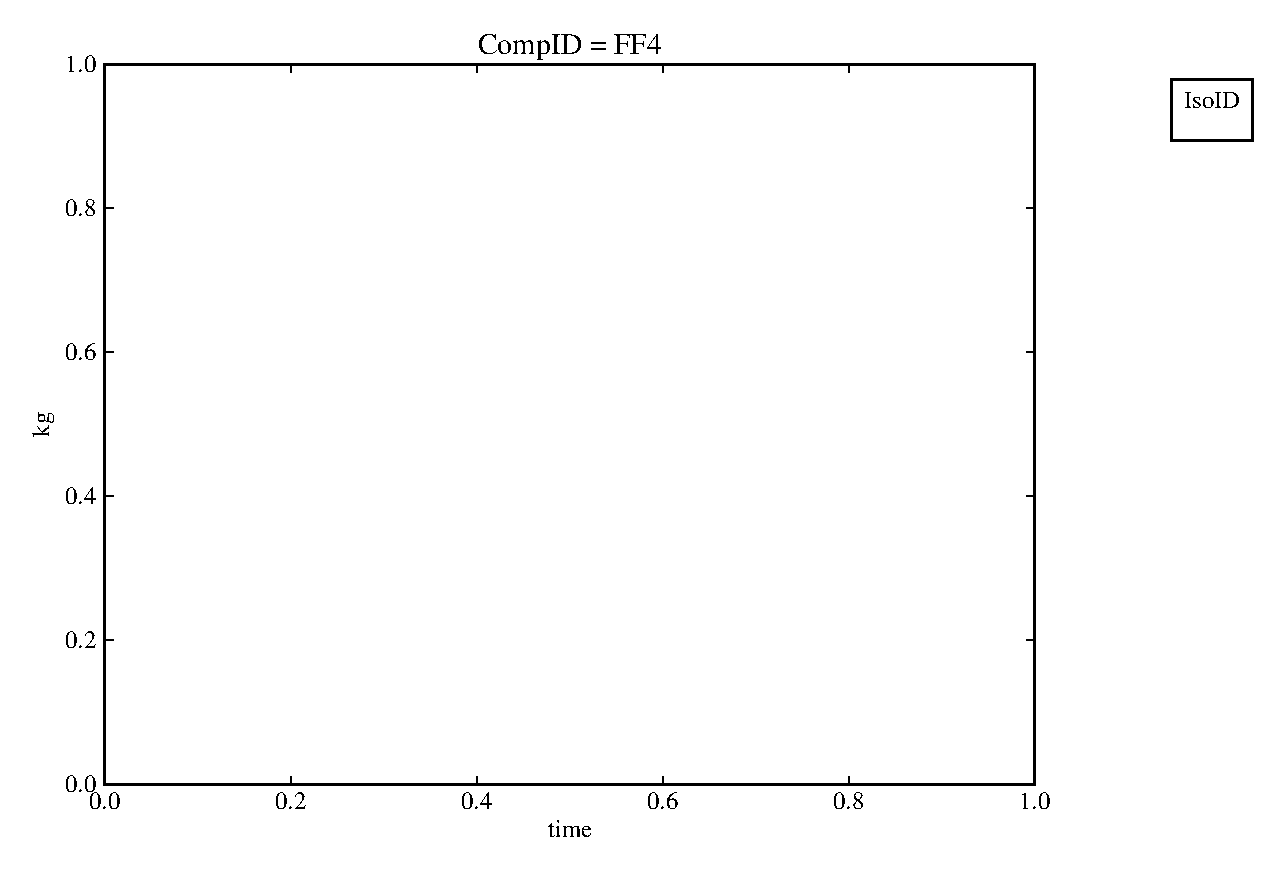
\includegraphics[width=\textwidth]{./chapters/demonstration/base/lpPFMII0.eps}
  \caption[Case LPPFMII Waste Package Contaminants.]{ 
    The Far Field, component 0 ($F_d = 0.1$), never recieves material.
    }
  \label{fig:lpPFMIIff0}
  \end{minipage}
\end{figure}
%\begin{figure}[ht]
%\centering
%\includegraphics[width=0.8\textwidth]{./chapters/demonstration/base/lpPFMIII.eps}
%\caption[$^{235}U$ residence. Lumped Parameter  <+Component+> No Release.]{
%For <+CASE+> case in which total containment in the <+component+> is assumed 
%($F_{d,<+comp+>}=0$), $^{235}U$ travels through  components ($F_d = 0.1$) before 
%permanent residence in the <+component+> component.
%}
%\label{fig:lpPFMIIIall}
%\begin{minipage}[b]{0.45\linewidth}
%
%  \includegraphics[width=\textwidth]{./chapters/demonstration/base/lpPFMIII1.eps}
%  \caption[LPPFMIII Waste Form Contaminants.]{
%    Waste Form 5 ($F_d = 0.1$) releases material with degradation. 
%    }
%  \label{fig:lpPFMIIIwf5}
%  
%  \includegraphics[width=\textwidth]{./chapters/demonstration/base/lpPFMIII3.eps}
%  \caption[Case LPPFMIII Buffer Contaminants]{
%    The Buffer, component 7 ($F_d=0$), acheives total containment.
%    }
%  \label{fig:lpPFMIIIbuff}
%
%\end{minipage}
%\hspace{0.05\linewidth}
%\begin{minipage}[b]{0.45\linewidth}
%  \includegraphics[width=\textwidth]{./chapters/demonstration/base/lpPFMIII2.eps}
%  \caption[Case LPPFMIII Waste Package Contaminants.]{ 
%    Waste Package 6 ($F_d = 0.1$) recieves then releases material. 
%    }
%  \label{fig:lpPFMIIIwp6}
%
%  \includegraphics[width=\textwidth]{./chapters/demonstration/base/lpPFMIII0.eps}
%  \caption[Case LPPFMIII Waste Package Contaminants.]{ 
%    The Far Field, component 0 ($F_d = 0.1$), never recieves material.
%    }
%  \label{fig:lpPFMIIIff0}
%
%
%  \end{minipage}
%\end{figure}
%\begin{figure}[ht]
%\centering
%\includegraphics[width=0.8\textwidth]{./chapters/demonstration/base/lpPFMIV.eps}
%\caption[$^{235}U$ residence. Lumped Parameter  <+Component+> No Release.]{
%For <+CASE+> case in which total containment in the <+component+> is assumed 
%($F_{d,<+comp+>}=0$), $^{235}U$ travels through  components ($F_d = 0.1$) before 
%permanent residence in the <+component+> component.
%}
%\label{fig:lpPFMIVall}
%\begin{minipage}[b]{0.45\linewidth}
%
%  \includegraphics[width=\textwidth]{./chapters/demonstration/base/lpPFMIV1.eps}
%  \caption[LPPFMIV Waste Form Contaminants.]{
%    Waste Form 5 ($F_d = 0.1$) releases material with degradation. 
%    }
%  \label{fig:lpPFMIVwf5}
%  
%  \includegraphics[width=\textwidth]{./chapters/demonstration/base/lpPFMIV3.eps}
%  \caption[Case LPPFMIV Buffer Contaminants]{
%    The Buffer, component 7 ($F_d=0$), acheives total containment.
%    }
%  \label{fig:lpPFMIVbuff}
%
%\end{minipage}
%\hspace{0.05\linewidth}
%\begin{minipage}[b]{0.45\linewidth}
%  \includegraphics[width=\textwidth]{./chapters/demonstration/base/lpPFMIV2.eps}
%  \caption[Case LPPFMIV Waste Package Contaminants.]{ 
%    Waste Package 6 ($F_d = 0.1$) recieves then releases material. 
%    }
%  \label{fig:lpPFMIVwp6}
%
%  \includegraphics[width=\textwidth]{./chapters/demonstration/base/lpPFMIV0.eps}
%  caption[Case LPPFMIV Waste Package Contaminants.]{ 
%    The Far Field, component 0 ($F_d = 0.1$), never recieves material.
%    }
%  \label{fig:lpPFMIVff0}
%
%
%  \end{minipage}
%\end{figure}
\FloatBarrier
